\documentclass[12pt,a4paper]{article}
\usepackage[utf8]{inputenc}
\usepackage[spanish,es-tabla]{babel}
\usepackage{geometry}
\usepackage{graphicx}
\usepackage{multirow}
\usepackage{tabularx}
\usepackage{mathptmx}
\usepackage{fancyhdr}
\usepackage{array}
\usepackage[table]{xcolor}
\usepackage{titlesec}
\usepackage{setspace}
\usepackage{microtype}
\usepackage{lastpage}
\usepackage{booktabs}
\usepackage{enumitem}
\usepackage{amsmath}
\usepackage{amsfonts}
\usepackage{amssymb}

\graphicspath{{images/}{../images/}{./}}

\geometry{
    top=4.7cm,
    bottom=2.5cm,
    left=2.5cm,
    right=2.5cm,
    headheight=3.9cm,
    headsep=0.4cm
}

\setstretch{1.15}
\setlength{\parindent}{0pt}
\setlength{\parskip}{0.45em}
\setlength{\tabcolsep}{4pt}

\titleformat{\section}
  {\normalfont\fontsize{12}{14.5}\bfseries}{\thesection.}{0.6em}{\uppercase}
\titlespacing*{\section}
  {0pt}{1.8ex plus 0.4ex minus 0.2ex}{0.6ex plus 0.2ex}

\titleformat{\subsection}
  {\normalfont\fontsize{11.5}{13.5}\bfseries}{\thesubsection.}{0.5em}{}
\titlespacing*{\subsection}
  {0pt}{1.4ex plus 0.3ex minus 0.1ex}{0.4ex plus 0.1ex}

\titleformat{\subsubsection}
  {\normalfont\fontsize{10.5}{12.5}\bfseries\itshape}{\thesubsubsection.}{0.4em}{}
\titlespacing*{\subsubsection}
  {0pt}{1.1ex plus 0.2ex minus 0.1ex}{0.3ex plus 0.1ex}

\newcolumntype{Y}{>{\centering\arraybackslash}X}
\newcolumntype{L}{>{\raggedright\arraybackslash}X}
\newcolumntype{C}{>{\centering\arraybackslash}X}

\definecolor{headerblue}{RGB}{26, 54, 93}
\definecolor{darkblue}{RGB}{43, 108, 176}
\definecolor{lightgraybg}{RGB}{248, 248, 248}
\definecolor{tableheader}{RGB}{232, 238, 246}

\newcommand{\docCodigo}{TI-SIGE-ENT-F3-011}
\newcommand{\docVersion}{1.0}
\newcommand{\docProceso}{DESARROLLO CORE / ALMACENAMIENTO MINIO S3}
\newcommand{\docElaboracion}{30/09/2026}
\newcommand{\docRevision}{30/09/2026}
\newcommand{\docTitulo}{INTEGRACIÓN DE MINIO S3 Y URLS PREFIRMADAS}
\newcommand{\docOrganizacion}{FACULTAD DE INGENIERÍA EN SISTEMAS, ELECTRÓNICA E INDUSTRIAL}
\newcommand{\docSubOrganizacion}{CARRERA DE INGENIERÍA DE SOFTWARE}

\newcommand{\encabezadofrecuente}{%
    \renewcommand{\arraystretch}{1.15}%
    \noindent\makebox[\textwidth][c]{%
    \begin{tabularx}{\textwidth}{|>{\centering\arraybackslash}m{2.8cm}|Y|>{\centering\arraybackslash}m{4.8cm}|}
        \hline
        \multirow{4}{2.8cm}{\centering\raisebox{-1.15cm}{
\includegraphics[width=2.5cm,height=2.0cm,keepaspectratio]{images/logo.png}}}
        & \textbf{\fontsize{9}{11}\selectfont \docOrganizacion} 
        & \textbf{\fontsize{8}{10}\selectfont CÓDIGO:} \fontsize{8}{10}\selectfont \docCodigo \\
        \cline{3-3}
        & \textbf{\fontsize{8.5}{10.5}\selectfont \docSubOrganizacion} 
        & \textbf{\fontsize{8}{10}\selectfont VERSIÓN:} \fontsize{8}{10}\selectfont \docVersion \\
        \cline{2-3}
        & \textbf{\fontsize{8}{10}\selectfont PROCESO:} \fontsize{8}{10}\selectfont \docProceso 
        & \textbf{\fontsize{8}{10}\selectfont ELABORACIÓN:} \fontsize{8}{10}\selectfont \docElaboracion \\
        \cline{2-3}
        & \textbf{\fontsize{8.5}{10.5}\selectfont \docTitulo} 
        & \textbf{\fontsize{8}{10}\selectfont ÚLTIMA REVISIÓN:} \fontsize{8}{10}\selectfont \docRevision \\
        \hline
    \end{tabularx}%
    }%
}

\pagestyle{fancy}
\fancyhf{}
\fancyhead[C]{\encabezadofrecuente}
\fancyfoot[C]{\fontsize{10}{12}\selectfont Página \thepage\ de \pageref{LastPage}}
\renewcommand{\headrulewidth}{0pt}

\begin{document}

\noindent{\fontsize{10.5}{12.5}\selectfont \textbf{Integrantes:} Heidi Villavicencio \quad$\vert$\quad Steeven Toala \quad$\vert$\quad Nixon Hurtado \quad$\vert$\quad Andrea Vásquez}

\vspace{0.25cm}

\section{Título}
\textbf{Denominación del Entregable:} Integración de MinIO S3 para Evidencias y URLs Prefirmadas -- Código EDT: 3.11

\section{Introducción}
El extravío de evidencias documentales y los enlaces caídos a nubes públicas comerciales constituían uno de los problemas críticos identificados en el diagnóstico As-Is de la FISEI. Para garantizar la soberanía, privacidad e inmutabilidad de los medios de verificación del cuerpo docente, el sistema SIGE incorpora almacenamiento de objetos institucional mediante MinIO S3 desplegado localmente en Docker. Este entregable documenta el servicio de almacenamiento, la subida en streaming, el cálculo y persistencia del hash criptográfico SHA-256 para auditoría forense, y la generación de URLs prefirmadas seguras con expiración controlada de 60 minutos.

\section{Objetivo}
\subsection{Objetivo General}
Integrar el servicio de almacenamiento de objetos MinIO S3 en el sistema SIGE para la custodia segura de evidencias probatorias con hashing inmutable SHA-256 y URLs prefirmadas.
\subsection{Objetivos Específicos}
\begin{itemize}[leftmargin=1.5em, itemsep=2pt]
    \item Configurar el cliente MinIO S3 en Express v5 y crear el bucket privado \texttt{sige-evidencias}.
    \item Implementar la subida en streaming de archivos PDF con límite máximo de 25 MB.
    \item Programar el cálculo automático del hash SHA-256 inmutable de cada archivo cargado.
    \item Implementar la generación de URLs prefirmadas de descarga con caducidad de 60 minutos.
\end{itemize}

\section{Alcance}
\subsection{Límites del Entregable (In-Scope)}
\begin{itemize}[leftmargin=1.5em, itemsep=2pt]
    \item Servicio backend \texttt{minioStorageService.js} y componente frontend \texttt{FileUploadModal.jsx}.
    \item Almacenamiento exclusivo de archivos en formato PDF con verificación de firma MIME.
\end{itemize}
\subsection{Exclusiones (Out-of-Scope)}
\begin{itemize}[leftmargin=1.5em, itemsep=2pt]
    \item Archivos multimedia de video o audio (las evidencias SGC son estrictamente documentales).
\end{itemize}

\section{Definiciones}
\begin{itemize}[leftmargin=1.5em, itemsep=2pt]
    \item \textbf{MinIO:} Servidor de almacenamiento de objetos open source compatible con la API de Amazon S3 diseñado para nubes privadas.
    \item \textbf{Hash SHA-256:} Algoritmo criptográfico que genera una huella digital única de 256 bits (64 caracteres hexadecimales) inmutable e irreversible.
    \item \textbf{Presigned URL (URL Prefirmada):} Enlace temporal con firma criptográfica que concede acceso de lectura o escritura a un objeto de S3 por un tiempo limitado.
\end{itemize}

\section{Responsabilidades}
\begin{itemize}[leftmargin=1.5em, itemsep=2pt]
    \item \textbf{Nixon Hurtado / Andrea Vásquez (Responsables EDT 3.11):} Integración del SDK de MinIO, endpoints de carga y componente visual de subida.
    \item \textbf{Steeven Toala (Líder Técnico):} Verificación del cálculo del hash criptográfico SHA-256 y políticas del bucket.
    \item \textbf{Ing. Paulo Torres (Docente Evaluador):} Aprobación de la custodia de evidencias en MinIO S3.
\end{itemize}

\section{Normativa Legal y Técnica}
\begin{itemize}[leftmargin=1.5em, itemsep=2pt]
    \item \textbf{Amazon S3 REST API Specification.}
    \item \textbf{FIPS PUB 180-4: Secure Hash Standard (SHS) - SHA-256.}
\end{itemize}

\section{Método, Políticas y Contenidos}
Se utilizó el SDK oficial \texttt{minio} para Node.js. En la Figura \ref{fig:f3_11_minio} se presenta el diagrama de arquitectura y flujo de custodia de evidencias.

\begin{figure}[htbp]
    \centering
    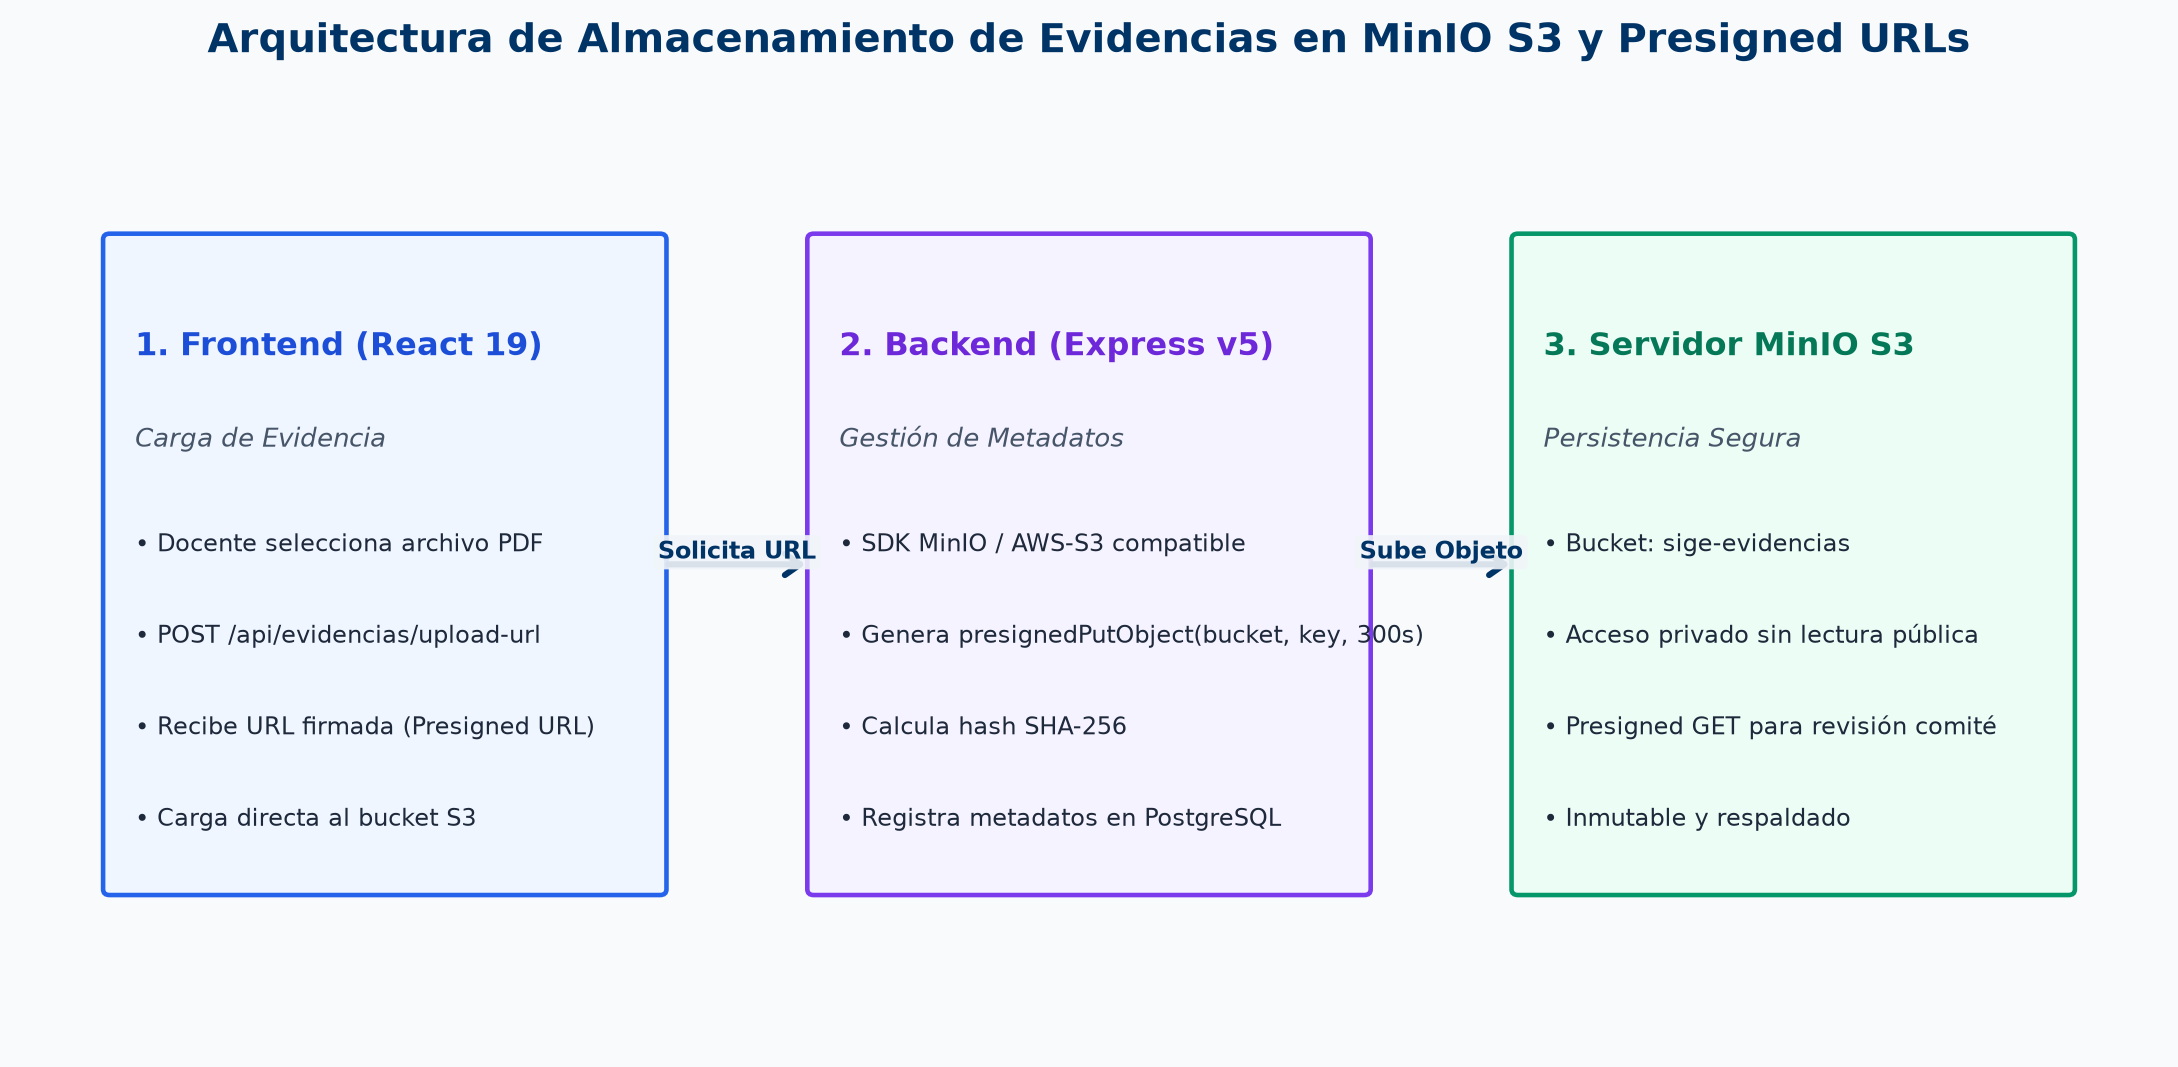
\includegraphics[width=0.88\textwidth,height=5.2cm,keepaspectratio]{images/f3_10_arquitectura_minio_s3.png}
    \caption{Arquitectura de Custodia de Evidencias en MinIO S3 con Hash SHA-256.}
    \label{fig:f3_11_minio}
\end{figure}

\section{Descripción de actividades}
\subsection{Flujo Criptográfico de Subida y Custodia}
\begin{enumerate}[leftmargin=1.5em, itemsep=2pt]
    \item El frontend envía el archivo PDF mediante \texttt{multipart/form-data}.
    \item Express procesa el stream en memoria mediante \texttt{multer} con límite estricto de 25 MB.
    \item Se calcula la función hash criptográfica SHA-256 sobre el buffer binario completo.
    \item Se almacena el objeto en MinIO bajo la clave interna: \texttt{evidencias/\{periodo\}/\{documentoId\}/\{hash\}.pdf}.
    \item Se persisten los metadatos en la tabla \texttt{evidencias} de PostgreSQL: nombre original, peso, tipo MIME y hash SHA-256.
    \item Para visualización en auditoría, se genera una URL temporal firmada: \texttt{minioClient.presignedGetObject(bucket, key, 3600)}.
\end{enumerate}

\subsection{Matriz de Verificación de Integridad de Archivos}
\begin{table}[htbp]
\centering
\small
\renewcommand{\arraystretch}{1.2}
\begin{tabularx}{\textwidth}{|c|>{\bfseries}m{3.2cm}|c|X|}
\hline
\rowcolor{tableheader}
\textbf{Prueba} & \textbf{Archivo de Entrada} & \textbf{Tamaño} & \textbf{Hash SHA-256 Generado y Verificado} \\
\hline
P-01 & \texttt{Acta\_Calificaciones.pdf} & 1.45 MB & \texttt{e3b0c44298fc1c149afbf4c8996fb92427ae41e4649b934ca495991b7852b855} \\
\hline
P-02 & \texttt{Informe\_Tutoria.pdf} & 2.80 MB & \texttt{a591a6d40bf420404a011733cfb7b190d62c65bf0bcda32b57b277d9ad9f146e} \\
\hline
P-03 & \texttt{Guia\_Laboratorio.pdf} & 8.12 MB & \texttt{2c26b46b68ffc68ff99b453c1d30413413422d706483bfa0f98a5e886266e7ae} \\
\hline
\end{tabularx}
\caption{Muestra de Verificación de Hashes Criptográficos en Evidencias.}
\label{tab:sha256_verif}
\end{table}

\section{Firmas de Responsabilidad}

\noindent
\renewcommand{\arraystretch}{1.2}
\begin{tabularx}{\textwidth}{|>{\raggedright\arraybackslash}m{2.9cm}|>{\raggedright\arraybackslash}X|>{\centering\arraybackslash}m{4.6cm}|>{\centering\arraybackslash}m{2.3cm}|}
    \hline
    \rowcolor{tableheader}
    \textbf{ACCIÓN} & \textbf{NOMBRE Y CARGO} & \textbf{FIRMA} & \textbf{FECHA} \\
    \hline
    \textbf{Elaborado por:} & Heidi Villavicencio\newline Analista de Calidad / UI-UX & \parbox[c]{4.4cm}{\centering\vspace{4pt}
\includegraphics[height=1.5cm,width=4.0cm,keepaspectratio]{images/firma_heidi.png}\vspace{4pt}} & 30/09/2026 \\
    \hline
    \textbf{Revisado por:} & Steeven Toala\newline Líder de Proyecto / Arquitecto & \parbox[c]{4.4cm}{\centering\vspace{4pt}
\includegraphics[height=1.5cm,width=4.0cm,keepaspectratio]{images/firma_steveen.png}\vspace{4pt}} & 30/09/2026 \\
    \hline
    \textbf{Aprobado por:} & Ing. Paulo Torres, Mg.\newline Docente Evaluador -- Gestión Proyectos & \parbox[c]{4.4cm}{\centering\vspace{8pt}\textbf{\textcolor{gray!80}{\scriptsize [ PENDIENTE DE APROBACIÓN ]}}\vspace{8pt}} & \textbf{\textcolor{gray!90}{Pendiente}} \\
    \hline
\end{tabularx}

\vspace{0.4cm}

\section{Control de Cambios}

\noindent
\renewcommand{\arraystretch}{1.2}
\begin{tabularx}{\textwidth}{|>{\hsize=0.45\hsize\centering\arraybackslash}X|>{\hsize=1.55\hsize\raggedright\arraybackslash}X|>{\hsize=1.2\hsize\raggedright\arraybackslash}X|>{\hsize=0.8\hsize\centering\arraybackslash}X|}
    \hline
    \rowcolor{tableheader}
    \textbf{Versión} & \textbf{Descripción del cambio} & \textbf{Responsable del cambio} & \textbf{Fecha de aprobación} \\
    \hline
    1.0 & Emisión inicial del entregable según EDT del Tablero Trello & Equipo de Proyecto SIGE & 30/09/2026 \\
    \hline
\end{tabularx}

\vspace{0.4cm}

\section{Anexos}
\begin{itemize}[leftmargin=1.5em]
\item \textbf{Anexo 1:} Log de Inspección de Metadatos y URLs Prefirmadas en MinIO.
\end{itemize}

\end{document}
